

\chapter{LITERATURE SURVEY}

\section{introduction:}

According to the World Federation of Deaf (WFD) \ref{} there are 70 million deaf people in world, whereas the world population in 2012 exceeded 7 billion \ref{}[4] , this number has got the power to make research in the field of machine vision  over  the  past  decade rich  approaches .
A  more  recent   technology  for gesture   recognition  is to  incorporate   the  information   of object   distances,   or depths,   normally   captured   by a 3D camera,   or a set  of cameras  that  produce 3D images and that it is Technology that will be used in this project  .It is also a contact-less  user interface,   in contrast   to glove-based   devices  or handhold   remote  sensor .
With the kinect DEpth Sensor stream data it is now possible to make recognize and  translate sign language in to speech and / or text in order to facilitate better communication between normal hearing and hearing impaired people. This is usually called Sign Language Recognition (SLR) which  aim  to automatically understand meaning of a sequence of signs from sign language without involvement of human interpreter \ref{ }. This chapter covers key aspects of SLR Literature .





\section{ Sign  Language Recognition}  

the SLR system can be divided into 4 important  steps , Data acquisition and feature extraction and finally Feature combination and Sign recognition .however in whats the next  we will cover Two important approaches that both  belongs to the first step ( Data acquisition ) :\\

Device based :

in  1991 Tomoichi Takahashi  \ref{ } developed a system for real-time SLR  using Device based approach such system required the user to wear gloves that were connected to computer for transmission of hand signal ,experiments showed that 34 of 46 gestures of the Japanese Kana manual alphabet were recognized correctly \ref{}.
 A wireless glove that was designed by Ryan Petters  \ref{}in 2002, sensed hand movements involved in sign language and then transmitted them wirelessly to portable device, that displayed translated signs as lines of text \ref{} [31].
 

vision based :

 This approach  \ref [32] here  feature extraction was done using color camera for recognition of ASL. Two experiments were run: the first required from the signer to wear colored gloves, while the second used hand’s skin color for feature extraction \ref [32]. The extracted features were used as input for HMM algorithm that was used during sign recognition phase. The first experiment attained 99\% word accuracy while the second 92\% \ref [32] .
 
 Two experiments were carried out also in \ref [33] on a SLR system that combined computer vision and HMM for recognition of sentence-level continuous ASL. Both systems were tested with forty (40) words from ASL, where in first systems single camera was mounted on desk to track user’s hands and achieved 92\% word accuracy, while in second system the user had to wear a cap worm in which camera was mounted and the achieved accuracy was 97\%  \ref [33].



We can Summarize The process Used in SLR literature as the following firgure \ref{} shows  :

\begin{figure}[H]
\centering
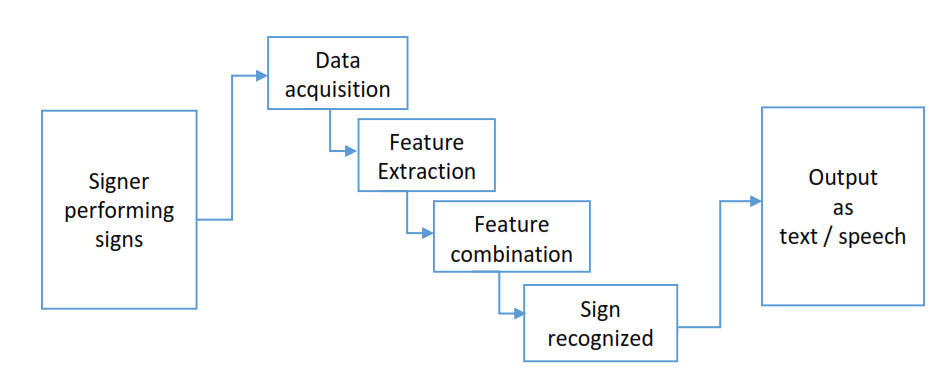
\includegraphics[width=0.6\textwidth]{img/SLR.PNG}
\caption{  process of SLR }
\label{fig:SLR}
\end{figure}

The presentation of all works related to SLR is not the intention of this section and more can be found on  \ref{}[27],\ref{} [36] and \ref{ }[39]. 

The following section present works that employed Kinect device for building SLR systems.Where we are going to discover The main ideas behind our project 

\section{Gesture Recognition Using Kinect :}

in \ref{} Zhou Ren et al presents a gesture recognition System using Kinect Sensor accompanied with a novel distance metric called Finger-Earth Mover’s Distance (FEMD) to measure the hand shape dissimilarities, which not only achieves better performance than Shape Context, in terms of accuracy (a 93.9\% mean accuracy) and efficiency (0.5004s).  \\

A more recent approach followed by Daniel in \ref{} uses Kinect skeletal tracking for features extraction. Other features were derived from skeletal tracking and finally 8-features were used for unique description of each sign. Sign recognition employs nearest neighbor algorithm that tries to find closest matching of performed sign within a group of stored sings  For a dictionary of 14 homemade signs the system achieves an accuracy of 95\% \ref{} [47].  \\

in \ref{} This paper presents an effective way of exploring depth information for hand gesture recognition. using  SIFT keypoint descriptor to extract local keypoint features
over depth images which is attempted for the first time in gesture recognition research. The recognition technique is inherently robust against scaling, rotation, and illumination conditions.  the features were  quantified  and clustered , and finally fed to  An SVM to be trained .\\


\mathbf{ Insipired HGR of This Project : }


\textbf{With \ref{} And \ref{} } we inspired our most work dedicated for this Project , we take advantage of  depth and Skeletal Tracking  data generated by Kinect to detect the hand and track it  in a range of [ 80 cm until 3 meters ] long  .
After detection of hand, we uses SURF Descriptor for Features detection and Extraction then we  cluster these vectors via a bag-of-features (BOW) model , these features are then Fed to an SVM with two different Kernels Linear and RBF kernel .\\

on the other hand unlike most system that like \ref{} that uses HMM ,  we proposed and tested a method for static hand gesture recognition.using  Fourier shape  descriptor which proved to be a very efficient way for feature extraction. It provided a set of invariant features for each image and by using a small number of features , we Found NN classifier to give faster and better results for Fourier descriptor .


\section{syntax}

....
\\
....
\\
....



\section{Conclusion}
